\chapter{Theoretical Framework\label{cha:chapter3}}
In existing systems, data streams are being consumed in the same form by their data users. It may be encrypted but not anonymized and in that way computers and people alike process the data. In this chapter, we lay the theoretical foundation for addressing the challenges and intricacies of anonymized access control in distributed event stores. Figure \ref{fig:theoretical_framework} shows the application of our solution. 

\begin{figure}[ht]
    \begin{adjustbox}{center}
    \includegraphics[width=0.73\pdfpagewidth]{img/Theoretical_framework.pdf}
    \end{adjustbox}
    \caption[Big picture of our solution to anonymizing data streams for the different data needs of its users.] {Our solution involves incorporating an anonymization system that transforms the input data stream into multiple anonymized versions, tailored to the specific data requirements of its users. The red numbers indicate the sequence of steps to configure the system. The green braces detail where we go into more detail about its components. \label{fig:theoretical_framework}}
\end{figure}

In its essence, the idea is to take the underlying data stream and anonymize it to fit the needs of each individual user group that interacts with it. In Figure \ref{fig:theoretical_framework} we include two data user groups - stream processors and employees. We want to indicate that both systems and humans process the data, and they often have very different tasks to accomplish. Identifying these data requirements is the task of, what we call, the Data Officer. They are responsible for the data management for the organization. As such they are familiar with the data flowing through the system and how each user group interacts with them. \par
Figure \ref{fig:theoretical_framework} includes a sequence of red numbers attached to the arrows originating from the Data Officer. They indicate the sequence of one-time actions that a Data Officer must perform to configure our proposed solution. First, 

\section{Managing Different Anonymization Granularity\label{sec:anon_granularity}}
When planning to integrate anonymization techniques into existing systems, there are many things to consider. First one must understand the data flowing through the system.
Does it include \ac{PII}? Is there further sensitive data? What part of it is necessary for system maintenance? Maybe there is additional data collected for statistics.
Bearing this in mind the next thought would be what needs to be anonymized. For this privacy agreements with the user must be taken into account. There may be additional government regulations in place like the \ac{CCPA} in the United States of America or the \ac{GDPR} in the European Union. 
The next course of action is deciding on specific masking functions. As was discussed in \ref{sec:anon} and further detailed in the subsequent section there is a plethora to choose from. It is important to note that all forms of anonymization lead to a loss of information. 
Choosing Blurring or Suppression, two methods that replace attributes with a placeholder, for all critical data fields derived in the previous assessment, will ensure that all privacy concerns are addressed, it will also diminish all intelligence gained from collecting this data in the first place. It is questionable if not collecting this type of data in the first place would then be the better solution as it would save storage and computing power. 
An alternative approach would be to invest heavily in IT security ensuring that no intruder with malicious intent can gain access to sensitive data. Keeping in mind, however, that social engineering attacks are nowadays the most common and effective strategy giving a guarantee of safety can be impossible. It also stands to reason that the more employees a company has the risk of social engineering attacks increases. Both of these radical approaches do not seem to adequately solve the problem. Fortunately, there is a way to navigate between these two extremes. An attentive observer of the company's data operations will likely notice that data can and should be restricted similarly to permissions: Only the data needed to fulfill the user's duty should be accessible to the user. 
In addition, there are anonymization techniques, which do not lead to total information loss like the two mentioned before. Generalization for example can be employed to significantly reduce the re-identification of individuals, while simultaneously retaining some information.
With data restriction and different anonymization techniques in mind, there is a middle ground to be found that maximizes security and minimizes information loss. Consider the following example:

\subsection{Use Case Example}
Hospitals depend on the collection, management, and analysis of data to administer the best and most accurate care to their patients. In a modern hospital, all data would be stored in a centralized hospital database. 
Here all data for individual patients are brought together. Table \ref{table:dia_patient} shows an exemplary table of patients in the endocrinology ward of a German hospital. Note that the tuple has been shortened to enhance its readability as well as prepended with a header of the corresponding database table. A more detailed version is shown in Table \ref{tab:patient_data} in Appendix A. 


\bigskip 


\begin{table}[ht]
    \begin{center}
    \footnotesize{
        \renewcommand{\arraystretch}{1.5}
        \begin{tabular}{ | c | c | c | c | c | c | c | c | c | c | c | } 
            \hline
            pid & name & zip & sex & age & ins. co. & ins. no. & diag. & gluc. & hba1c & med. \\
            \hline
            1 & F. Ott & 10969 & M & 28 & TK & K15489 & E10 & 22.1 & 8.74 & Insulin \\
            \hline
            2 & L. Lieb & 34127 & F & 59 & AOK & Y41271 & E11 & 16.3 & 7.61 & Metformin \\
            \hline 
            3 & T. Zeit & 70192 & M & 15 & TK & Z17291 & E10 & 23.8 & 8.13 & Insulin \\
            \hline
            4 & H. Lang & 80923 & F & 21 & TK & I79435 & E10 & 18.9 & 7.99 & Insulin \\
            \hline
            5 & J. Putz & 91757 & D & 24 & IKK & Q29751 & E10 & 21.2 & 6.04 & Insulin \\
            \hline
            6 & I. Spies & 60819 & M & 68 & TK & J33921 & E11 & 19.1 & 5.07 & Metformin \\
            \hline
        \end{tabular}
    }
    \caption{Example table of diabetes patients}
    \label{table:dia_patient}
    \end{center}
\end{table}

The header of table \ref{table:dia_patient} shows eleven attributes. First the person id (\textit{pid}), which is the primary key for each patient as it uniquely identifies the patient in the database. Then \textit{name}, zip code (\textit{zip}), \textit{sex} and \textit{age} are included as additional personal information.
This would typically also include the full address not just the zip code, contact information, height as well as weight to adapt the dosage of the medication. The subsequent two attributes include information about the patient's insurance information. 
Insurance companies in Germany are uniquely identified with a nine-digit institutional identifier. In the case of the first entry the insurance company (\textit{ins. co.}) has the value 101575519, which matches the identifier of the Techniker Krankenkasse (TK). 
Each client is then assigned a number unique to that insurance company called the insurance number (\textit{ins. no.}). It always starts with a letter followed by digits. Finally, the datum references the medical information. It starts with the diagnosis (\textit{diag.}) classified according to the \ac*{ICD}. 
E10 is the label for Type 1 Diabetes Mellitus; E11 is the label for Type 2 Diabetes Mellitus. The most important medical measurement for the treatment of this disease is the current amount of glucose (\textit{gluc.}) in the blood. This determines the quantity of medication (\textit{med.}) to be administered to the patient. For Type 1 Diabetes this is Insulin, for Type 2 it is Metformin. 
Lastly, the table includes an attribute called \textit{hba1c}. This is the body's three-month average of blood glucose. Through which diabetes is diagnosed. In this case, it is also symbolic for all additional diagnostic findings. 
Glucose and HbA1c are intentionally distinguished as separate attributes in this dataset, despite both being blood-derived metrics, due to their distinct measurement methodologies and relevance in immediate treatment contexts. Glucose can be ascertained with a single drop of blood, providing critical information for immediate treatment.
Conversely, HbA1c is derived from a complete blood count and does not require instant action. \par

In a hospital setting, numerous actors engage with the aforementioned dataset. The most straightforward and prominent is the doctor. She will need all data to fulfill her duties. The doctor's letter contains all personal information. The medical data is needed for diagnosis and treatment. 
She will also need to keep the insurance information in mind as the covered treatment options are oftentimes different for each company. Additionally, she will need to write the patient's insurance information on the prescriptions. Only the pid could be omitted, but is debatable if the overhead is worth it, considering the pid can be easily inferred with all the given information.
Therefore, no anonymization of the doctor's data makes the most sense. \par

Supporting the doctor is the nurse staff. One of their main tasks is to monitor patients and administer medication. To accomplish this they require the diagnosis, medication, and in this case the glucose data. As the HbA1c value is not relevant for the immediate treatment it can be safely omitted. 
Again insurance information is necessary as nurses typically do have the liberty to administer medication according to their judgment. This is especially important when considering how understaffed hospitals in Germany are most of the time. On the other hand, the patient's insurance number does not play into this. As nurses also interact directly with the patients they need some basic personal information like name and sex. 
Pid and zip, however, are not required. Therefore, the data for the nurse staff can be anonymized as shown in Table \ref{table:nurse} without limiting the nurses or losing valuable information. 

\bigskip

\begin{table}[ht]
    \begin{center}
    \footnotesize{
        \renewcommand{\arraystretch}{1.5}
        \begin{tabular}{ | c | c | c | c | c | c | c | c | c | c | c | } 
            \hline
            \cellcolor{lightred} pid & name & \cellcolor{lightred} zip & sex & age & ins. co. & \cellcolor{lightred} ins. no. & diag. & gluc. & \cellcolor{lightred} hba1c & med. \\
            \hline
            \cellcolor{lightred} * & F. Ott & \cellcolor{lightred} * & M & 28 & TK & \cellcolor{lightred} * & E10 & 22.1 & \cellcolor{lightred} * & Insulin \\
            \hline
            \cellcolor{lightred} * & L. Lieb & \cellcolor{lightred} * & F & 59 & AOK & \cellcolor{lightred} * & E11 & 16.3 & \cellcolor{lightred} * & Metformin \\
            \hline 
            \cellcolor{lightred} * & T. Zeit & \cellcolor{lightred} * & M & 15 & TK & \cellcolor{lightred} * & E10 & 23.8 & \cellcolor{lightred} * & Insulin \\
            \hline
            \cellcolor{lightred} * & H. Lang & \cellcolor{lightred} * & F & 21 & TK & \cellcolor{lightred} * & E10 & 18.9 & \cellcolor{lightred} * & Insulin \\
            \hline
            \cellcolor{lightred} * & J. Putz & \cellcolor{lightred} * & D & 24 & IKK & \cellcolor{lightred} * & E10 & 21.2 & \cellcolor{lightred} * & Insulin \\
            \hline
            \cellcolor{lightred} * & I. Spies & \cellcolor{lightred} * & M & 68 & TK & \cellcolor{lightred} * & E11 & 19.1 & \cellcolor{lightred} * & Metformin \\
            \hline
        \end{tabular}
    }
    \caption{Data available for the nurse staff. Note that PID, zip, insurance number, and additional medical information have been suppressed as indicated by their cell's light red background.}
    \label{table:nurse}
    \end{center}
\end{table}

In tandem with the stay and medical treatment of the patient, the administration of the hospital will want to collect the money from the patient's insurance. The insurance company together with the patient's personal insurance number will suffice as identification. 
Administered medication will be imperative as this dictates the amount of money the hospital will get in addition to the fees for the stay. For this, the diagnosis will typically have to be added as a suitable reason. No further information is required. Limiting the amount of data here 
is crucial as the data is exported to a third party. Which means that additional regulations will take effect. Minimizing the data leaving the hospital minimizes security risks. With these strict rules in place, the data can be adjusted as seen in Table \ref{table:administration}. \newline 
Note at this point that an unauthorized entity, who has gained access to both the data of the nurse staff and that of the administration, would struggle to correlate the entries. The shared available data fields insurance company, diagnosis, and medication are likely generic enough to not point to a singular but to many patients. 

\bigskip

\begin{table}[ht]
    \begin{center}
    \footnotesize{
        \renewcommand{\arraystretch}{1.5}
        \begin{tabular}{ | c | c | c | c | c | c | c | c | c | c | c | } 
            \hline
            \cellcolor{lightred} pid & \cellcolor{lightred} name & \cellcolor{lightred} zip & \cellcolor{lightred} sex & \cellcolor{lightred} age & ins. co. & ins. no. & diag. & \cellcolor{lightred} gluc. & \cellcolor{lightred} hba1c & med. \\
            \hline
            \cellcolor{lightred} * & \cellcolor{lightred} * & \cellcolor{lightred} * & \cellcolor{lightred} * & \cellcolor{lightred} * & TK & K15489 & E10 & \cellcolor{lightred} * & \cellcolor{lightred} * & Insulin \\
            \hline
            \cellcolor{lightred} * & \cellcolor{lightred} * & \cellcolor{lightred} * & \cellcolor{lightred} * & \cellcolor{lightred} * & AOK & Y41271 & E11 & \cellcolor{lightred} * & \cellcolor{lightred} * & Metformin \\
            \hline 
            \cellcolor{lightred} * & \cellcolor{lightred} * & \cellcolor{lightred} * & \cellcolor{lightred} * & \cellcolor{lightred} * & TK & Z17291 & E10 & \cellcolor{lightred} * & \cellcolor{lightred} * & Insulin \\
            \hline
            \cellcolor{lightred} * & \cellcolor{lightred} * & \cellcolor{lightred} * & \cellcolor{lightred} * & \cellcolor{lightred} * & TK & I79435 & E10 & \cellcolor{lightred} * & \cellcolor{lightred} * & Insulin \\
            \hline
            \cellcolor{lightred} * & \cellcolor{lightred} * & \cellcolor{lightred} * & \cellcolor{lightred} * & \cellcolor{lightred} * & IKK & Q29751 & E10 & \cellcolor{lightred} * & \cellcolor{lightred} * & Insulin \\
            \hline
            \cellcolor{lightred} * & \cellcolor{lightred} * & \cellcolor{lightred} * & \cellcolor{lightred} * & \cellcolor{lightred} * & TK & J33921 & E11 & \cellcolor{lightred} * & \cellcolor{lightred} * & Metformin \\
            \hline
        \end{tabular}
    }
    \caption{Data available for the administration. Note that only the insurance information, medication, and diagnosis are not suppressed.}
    \label{table:administration}
    \end{center}
\end{table}

Diabetes, which afflicts over ten percent of the global population and demonstrates a rising prevalence, stands as one of the most common chronic diseases worldwide \cite{idf2023, WHODiabetes2023}. Given its mostly non-lethal progression and lifetime dependency on medication, 
it has given rise to a substantial market. As the cause, optimal treatment, and cure remain subject to research, data from especially newer diabetes patients is in hot demand. To provide this data to research institutes following the regulations in place the hospital must ensure that no concrete patient can be reidentified. 
Here, advanced anonymization techniques such as K-Anonymization come into play. Each attribute of the data entry can be assigned to one of three categories: personally identifiable, quasi-identifying, and sensitive attributes. To achieve k-anonymity each entry must suppress the personally identifiable attributes - while keeping the sensitive attributes untouched. 
Most importantly the quasi-identifiable attributes of each data entry must be the same for at least k - 1 other entries of a data set. This is typically achieved with generalization of these attributes until k entries are found. In this use case, the personally identifiable attributes are \textit{pid}, \textit{name}, and \textit{insurance number}. 
The quasi-indentifying attributes are \textit{zip}, \textit{sex}, \textit{age}, and \textit{insurance company}. The medical data comprises sensitive attributes. A K anonymous version of this data extry is depicted in Table \ref{table:k_anon}. 

\bigskip

\begin{table}[ht]
    \begin{center}
        \footnotesize{
            \renewcommand{\arraystretch}{1.5}
            \begin{adjustbox}{center}
                \begin{tabular}{ | c | c | c | c | c | c | c | c | c | c | c | } 
                    \hline
                    \cellcolor{lightred} pid & \cellcolor{lightred} name & \cellcolor{lightyellow} zip & \cellcolor{lightyellow} sex & \cellcolor{lightyellow} age & \cellcolor{lightyellow} ins. co. & \cellcolor{lightred} ins. no. & diag. & gluc. & hba1c & med. \\
                    \hline
                    \cellcolor{lightred} * & \cellcolor{lightred} * & \cellcolor{lightyellow} XXXXX & M & \cellcolor{lightyellow} {[10 - 70]} & TK & \cellcolor{lightred} * & E10 & 22.1 & 8.74 & Insulin \\
                    \hline
                    \cellcolor{lightred} * & \cellcolor{lightred} * & \cellcolor{lightyellow} XXXXX & M & \cellcolor{lightyellow} {[10 - 70]} & TK & \cellcolor{lightred} * & E10 & 23.8 & 8.13 & Insulin \\
                    \hline 
                    \cellcolor{lightred} * & \cellcolor{lightred} * & \cellcolor{lightyellow} XXXXX & M & \cellcolor{lightyellow} {[10 - 70]} & TK & \cellcolor{lightred} * & E11 & 19.1 & 5.07 & Metformin \\
                    \hline
                    \cellcolor{lightred} * & \cellcolor{lightred} * & \cellcolor{lightyellow} XXXXX & \cellcolor{lightyellow} \{M, F, D\} & \cellcolor{lightyellow} {[10 - 70]} & \cellcolor{lightyellow} ins. co. & \cellcolor{lightred} * & E11 & 16.3 & 7.61 & Metformin \\
                    \hline
                    \cellcolor{lightred} * & \cellcolor{lightred} * & \cellcolor{lightyellow} XXXXX & \cellcolor{lightyellow} \{M, F, D\} & \cellcolor{lightyellow} {[10 - 70]} & \cellcolor{lightyellow} ins. co. & \cellcolor{lightred} * & E10 & 18.9 & 7.99 & Insulin \\
                    \hline
                    \cellcolor{lightred} * & \cellcolor{lightred} * & \cellcolor{lightyellow} XXXXX & \cellcolor{lightyellow} \{M, F, D\} & \cellcolor{lightyellow} {[10 - 70]} & \cellcolor{lightyellow} ins. co. & \cellcolor{lightred} * & E10 & 21.2 & 6.04 & Insulin \\
                    \hline
                \end{tabular}
            \end{adjustbox}
        }
    \caption{K-anonymized data available for external research. The sensitive medical attributes remain unchanged as indicated by the white cell background. Unlike the personally identifying attributes, which have been suppressed as denoted by the red cell background. The yellow cell background highlights the generalized quasi-identifiable attributes. Note that the entries of the first group have unchanged values for the attributes \textit{sex} and \textit{ins. co.}. As all three original entries shared the same value it did not need to be generalized.}
    \label{table:k_anon}
    \end{center}
\end{table}

While the aforementioned diabetes patient use case scenario may appear unique and specific, the aspects and nuances are applicable in numerous contexts. The distinct data requirements for doctors, nurses, administration, and research are anticipated to persist, albeit adapted, throughout the entire healthcare industry. 
It is also viable in different sectors. Imagine security levels in government matters, trade secrets, and specific customer knowledge in corporations or secrecy of correspondence for the transportation industry. Distributed event stores are utilized across all of these sectors with major players relying on distributed event stores for their everyday needs \cite{kafka}. 

\section{Anonymization Techniques Classification\label{sec:anonymization_hierarchy}}
Data anonymization is a multifaceted process tailored to meet diverse application requirements and user needs. This section first categorizes the anonymization techniques based on their scope of operation, simultaneously setting them into context with each other through a hierarchical structure. It will then continue to go in-depth on each category, highlighting the intricacies of that category alone and providing insights, implementation considerations, and use cases to prominent examples. The aim is to provide a structured understanding of their application in various contexts.\par

We delineate the categorization of anonymization techniques as follows: 

\begin{itemize}
    \item \textbf{Value-Based} Handles one tuple at a time and replaces the values of attributes independently. 
    \item \textbf{Tuple-Based} Operates on individual attributes of a single tuple - but considers the values of the entire tuple for the change. 
    \item \textbf{Attribute-Based} Extends the view from one tuple to a larger collection or table of data. Evaluate the values of singular attributes of the entire set and collectively make changes to that attribute accordingly. 
    \item \textbf{Table-Based} Covers a table of data and perceives all attributes of each tuple. Adaptions to multiple attributes simultaneously are common. It can be argued that methods falling under this category are not masking functions but algorithms utilizing many masking functions to achieve anonymization on a table level.  
\end{itemize}

To better illuminate the relationship and hierarchy of the aforementioned categories as well as provide some examples, refer to Figure \ref{fig:hierarchy_mf}. These categorizations are critical for selecting suitable anonymization strategies in various real-world applications. Having outlined the structure and dimensions of the various masking functions, it is now time to take a closer look at the functionality and use cases, beginning with the value-based masking functions. 

\begin{figure}[ht]
    \begin{tikzpicture}[node distance=1.5cm, auto, trim left=-2.5cm]
        % Define block styles
        \tikzstyle{box} = [rectangle, draw, rounded corners, fill=blue!20, text width=5em, text centered, minimum height=3em]
        \tikzstyle{line} = [draw, -latex']

        % Nodes
        
        \node [box, text width=5em, xshift=-1cm] (value) {Value Based};
        \node [box, right=of value, text width=5em] (tuple) {Tuple Based};
        \node [box, right=of tuple, text width=6em] (attribute) {Attribute Based};
        \node [box, right=of attribute, text width=5em] (table) {Table Based};
        \node [box, fill=purple!30, above=of tuple, text width=9em] at ($(value)!0.5!(tuple)$) (semantics1) {Tuple-at-the-time\\ Semantics};
        \node [box, fill=purple!30, above=of attribute, text width=6em] at ($(attribute)$) (semantics2) {Table Semantics};
        \node [box, fill=purple!50, above=of semantics1, text width=6em] at ($(semantics1)!0.5!(semantics2)$) (masking) {Masking Functions};
        \node [box, fill=white, text width=6em, opacity=0, above=of table] at ($(table)$) (reference){};
        \node [box, fill=green!30, above=of reference, text width=7.5em] at ($(reference)$) (anonymizations) {Table Anonymizations};


        % Lists
        \node[below=0.2cm of value] (value_mf) {
            \begin{tabular}{l}
                - Suppression \\
                - Blurring \\
                - Substitution \\
                - Tokenization \\
                - Generalization \\
                - Bucketizing \\
                - Noise Methods
            \end{tabular}
        };

        \node[below=0.2cm of tuple] (tuple_mf) {
            \begin{tabular}{l}
                - Conditional \\ Substitution
            \end{tabular}
        };

        \node[below=0.2cm of attribute] (attribute_mf) {
            \begin{tabular}{l}
                - Aggregation \\
                - Univariate \\ Microaggregation \\
                - Shuffling 
            \end{tabular}
        };

        \node[below=0.2cm of table] (table_mf) {
            \begin{tabular}{l}
                - k-anonymization \\
                - l-diversity \\
                - t-closeness \\
                - Multivariate \\ Microaggregation 
            \end{tabular}
        };

        % Paths
        \path [line] (masking) -- (semantics1);
        \path [line] (masking) -- (semantics2);
        \path [line] (semantics1) -- (value);
        \path [line] (semantics1) -- (tuple);
        \path [line] (semantics2) -- (attribute);
        \path [line] (anonymizations) -- (table);

    \end{tikzpicture}
    \vspace{-0.75cm}
    \caption{Hierarchy of masking functions}\label{fig:hierarchy_mf} 
\end{figure}

\subsection{Value-Based Masking Functions}
Value-based masking functions form the foundation of data anonymization. These functions focus on altering single values within a tuple. They play a pivotal role in the construction of more complex anonymization methods. Although integral, their application in isolation often falls short of providing robust protection, due to their limited scope of operation, which is restricted to a single attribute. Utilizing them together in the context of more complex anonymization strategies is essential in providing effective data protection. In Section \ref{sec:masking_functions} we have already covered these simple masking functions and refer the reader to that for more detail. For the sake of completeness and quick reference, we provide a short overview of the most prominent value-based masking functions: 

\begin{itemize}
    \item \textbf{Suppression} Replaces a value with a generic value.
    \item \textbf{Blurring} Alters a value by partial suppression.
    \item \textbf{Substitution} Replaces one value with another valid value given a lookup table.
    \item \textbf{Tokenization} Replaces one value with a random value. The mapping is stored in a database.
    \item \textbf{Generalization} Generalizes a value using a predefined generalization hierarchy. 
    \item \textbf{Bucketizing} Specialized version of Generalization referring to numerical values. They are generalized by discretizing the value range and replacing each value with the corresponding range. 
    \item \textbf{Noise Methods} Adds noise to each value, where the noise can be additive or multiplicative.
\end{itemize}


\subsection{Tuple-Based Masking Functions}
Extending the scope of operation from independent attributes to the tuple as a whole yields the tuple-based masking functions. The most notable candidate is \textbf{Conditional Substitution}. As can be expected the change to the tuple is identical to that of the value-based Substitution. The value of the attribute specified by the parameter is changed according to the given substitution dictionary. The key difference, however, is that a change only occurs if a certain condition is met. These are additionally provided as a parameter. They can be specified in a variety of different possible formats like a direct match, a numerical range, or even a regular expression. Before showcasing some examples consider the following definitions: \par

Let $T$ be a tuple defined as a fixed sequence of attributes $a_0$ to $a_n$, $T = (a_0, a_1, \dots, a_n)$. Also, let $i$, $j$ $\in \{0,1, \dots, n\}$. \par

Further, a masking function for conditional substitution $mf_{cs}$ can be defined based on a condition $c$ evaluated on the attribute $a_i$, with a substitute $s$ for the attribute $a_j$:
\vspace{-0.8em}
\[
\begin{aligned}
mf_{cs}(i, c, j, s) &= 
\begin{cases}
    (a_0, \dots, a_{j-1}, s, a_{j+1}, \dots, a_n) & \text{if } c \text{ matches on } a_i \\
    T & \text{else}
\end{cases}
\end{aligned}
\]

Note, that a match on c can take on different forms. An example of a conditional substitution masking function for a direct match on the value of one of the attributes is shown in Figure \ref{fig:condiSubValue}. It shows an excerpt of a database table with three entries. Remember that all tuples of a single database table share the same data scheme. For better understanding, the header with the attribute's labels is shown in the first row of each table in the figure. It shows that the data in this table has two attributes, \textit{rank} and \textit{salary}. The masking function $mf_{cs}(0, 'Manager', 1, '*')$ is applied to every tuple in the table. It can be read as: if the attribute with index 0 matches on 'Manager', substitute the attribute with index 1 with '*'. Following this logic only one entry in the output was changed, as there was just one match.

\bigskip

\begin{figure}[ht]
    \begin{center}
    \footnotesize{
        \renewcommand{\arraystretch}{1.5}
        \begin{tabular}{|c|c|}
            \hline
            rank & salary\\
            \hline
            Worker & 62 000 \\
            \hline
            Assistant & 45 000 \\
            \hline
            Manager & 135 000 \\
            \hline
        \end{tabular}
        \quad $\xrightarrow{mf_{cs}(0, 'Manager', 1, '*')}$ \quad
        \begin{tabular}{|c|c|}
            \hline
            rank & salary\\
            \hline
            Worker & 62 000 \\
            \hline
            Assistant & 45 000 \\
            \hline
            Manager & * \\
            \hline
        \end{tabular}
    }
    \end{center}
    \caption{Conditional substitution with a direct match condition taking the entire tuple into consideration.\label{fig:condiSubValue}}
\end{figure}

Another example is shown in Figure \ref{fig:condiSubRange}. The condition in this case is a range. Naturally, it can only be applied to numerical attributes since there is a clear ordering of values. In the example, the database table shows two attributes: \textit{name} and \textit{age}. The masking function employed is $mf_{cs}(1,[0, 18], 1, 'minor')$. Subsequently, the output shows two changes in the table as two entries match the condition. Note that this time the condition is evaluated on the same attribute as the substitution e.g. $i = j$. 


\bigskip

\begin{figure}[ht]
    \begin{center}
    \footnotesize{
        \renewcommand{\arraystretch}{1.5}
        \begin{tabular}{|c|c|}
            \hline
            name & age \\
            \hline
            John & 45 \\
            \hline
            Frederik & 7 \\
            \hline
            Samatha & 15 \\
            \hline
        \end{tabular}
        \quad $\xrightarrow{mf_{cs}(1,[0, 18], 1, 'minor')}$ \quad
        \begin{tabular}{|c|c|}
            \hline
            name & age \\
            \hline
            John & 45 \\
            \hline
            Frederik & minor  \\
            \hline
            Samatha & minor \\
            \hline
        \end{tabular}
    }
    \end{center}
    \caption{Substitution with a range condition on the basis of only a singular attribute in the tuple. \label{fig:condiSubRange}}
\end{figure}

Finally, Figure \ref{fig:condiSubRegex} shows $mf_{cs}(0,'@example\backslash.com', 1, 0)$ being used as masking function. The attribute \textit{Points} for all entries with the domain 'example.com' in the \textit{Email} attribute, determined through the regular expression \textit{$'@example\backslash.com'$} is set to 0. 

\bigskip

\begin{figure}[ht]
    \begin{center}
    \footnotesize{
        \renewcommand{\arraystretch}{1.5}
        \begin{tabular}{|c|c|}
            \hline
            Email & Points \\
            \hline
            user1@example.com & 150 \\
            \hline
            service@mail.org & 325 \\
            \hline
            john@example.com & 25 \\
            \hline
        \end{tabular}
        \quad $\xrightarrow{mf_{cs}(0,'@example\backslash.com', 1, 0)}$ \quad
        \begin{tabular}{|c|c|}
            \hline
            Email & Points \\
            \hline
            user1@example.com & 0 \\
            \hline
            service@mail.org & 325 \\
            \hline
            john@example.com & 0 \\
            \hline
        \end{tabular}
    }
    \end{center}
    \caption{Regular expression as a condition for the substitution as part of a tuple-based masking function. \label{fig:condiSubRegex}}
\end{figure}

\subsection{Attribute-Based Masking Functions}
Following the hierarchy of masking functions depicted in Figure \ref{fig:hierarchy_mf} this concludes the masking functions with Tuple-at-the-time semantics. Next, the focus shifts towards operations on tables, more specifically on collections of tuples. Before, the masking functions were applied to each tuple individually. The focus is to add more context to the anonymization and in return diminish the information loss caused by anonymizing altogether. Also, it allows the better handling of outliers. Returning to the generalization example from Figure \ref{fig:generalization}, where the residency 'Berlin' was generalized to 'Germany'. If in an entire table there is only one German resident, it would be easy for an unauthorized party, who has gained access to this table, to reidentify the individual from the output. All the masking operation would have done is cost resources and lead to information loss within the system. This is of course not desirable. Fortunately, edge cases like these are unlikely for data with low spread or high density. Even in data sets with high spread and the likelihood of outliers, situations like the aforementioned can be easily avoided with knowledge of the data and the correct choice of masking function for the appropriate edge cases e.g. Suppression. An approach that more complex anonymization techniques like the ones discussed in Section \ref{lit:data_streaming} employ inherently. The subsequent subsection will go into more depth on this as well. For the moment, it is crucial to understand that more input can lead to less information loss and more anonymization reliability. It does, however, come at a higher computing cost as the findings in Chapter \ref{cha:chapter5} show. More input in the context of attribute-based masking functions refers to more values from multiple tuples for the same attribute. Within the scope of this thesis, it is essential to highlight the particular interest in data streams being the foundation of distributed event stores as opposed to static databases or bounded datasets. Data streams inherently pose additional challenges due to their unbounded nature. In Section \ref{lit:data_streaming} this has been addressed already and windowing was introduced as a means of discretizing data streams. In this context 'collections of tuples', 'table', and 'window' all refer to this same discretization: a finite number of tuples as a working base obtained through windowing operations. It is worth mentioning that the parameters for windowing like window size can be included in the optimization of the anonymization itself. This particular nuance is looked into in Section \ref{sec:parameterOptimization} \par

Building on this understanding, \textbf{Aggregation} as an attribute-based masking function leverages this principle. In essence, aggregation combines multiple values into one single value. This in turn will represent the attribute for all input tuples. This effectively reduces the information of an individual entry but preserves the underlying trend. By merging data it significantly reduces the reidentification probability of a single individual through this attribute. There is a variety of aggregation techniques, but they all have one thing in common. They work only on numerical values. Figure \ref{fig:aggregation} shows an example. The table contains six tuples, each tuple only has one attribute, \textit{age}. The right side of the arrow illustrates the result. Note that the amount of tuples remains unchanged, but now all tuples have the same value for the attribute. Depending on the aggregation type, which is written underneath each column, the values have been combined. The first column shows the sum, the second the median, the third the average, the fourth the maximum value found, the fifth the minimum value found, the sixth the number of input tuples, and the last the most frequent value in the input table. 

\bigskip

\begin{figure}[ht]
    \begin{center}
    \footnotesize{
        \renewcommand{\arraystretch}{1.5}
        \begin{tabular}{|*{1}{C{1.2cm}|}}
            
            \hline
            age \\
            \hline
            23 \\
            \hline
            45  \\
            \hline
            26 \\
            \hline
            32  \\
            \hline
            26 \\
            \hline
            27 \\
            \hline
            \multicolumn{1}{c}{} \\
        \end{tabular}
        \quad $\longrightarrow$ \quad
        \begin{tabular}{|*{7}{C{1.2cm}|}}
            \hline
            \multicolumn{7}{|c|}{age} \\
            \hline 
            180 & 32 & 30 & 45 & 23 & 6 & 26 \\
            \hline
            180 & 32 & 30 & 45 & 23 & 6 & 26 \\
            \hline
            180 & 32 & 30 & 45 & 23 & 6 & 26 \\
            \hline
            180 & 32 & 30 & 45 & 23 & 6 & 26 \\
            \hline
            180 & 32 & 30 & 45 & 23 & 6 & 26 \\
            \hline
            180 & 32 & 30 & 45 & 23 & 6 & 26 \\
            \hline
            \multicolumn{1}{c}{Sum} & \multicolumn{1}{c}{Median} & \multicolumn{1}{c}{Average} & \multicolumn{1}{c}{Max} & \multicolumn{1}{c}{Min} & \multicolumn{1}{c}{Count} & \multicolumn{1}{c}{Mode} \\
            
        \end{tabular}
    }  
    \end{center}
    \caption{Aggregation operations on the "age" attribute.\label{fig:aggregation}}
\end{figure}

A special form of aggregation is \textbf{Univariate Microaggregation\label{lit:univariate}}. This masking function specifically optimizes the goal of minimizing information loss. The method accomplishes this by clustering similar data. The aggregation is then only applied to these groups. This approach yields a table with greater variance in data than what is observed with standard aggregation. Also, outliers have less effect on the overall table. Of course, the clustering of data will require additional resources. One approach to univariate microaggregation is offered by Hansen and Mukherjee \cite{HansenUnivariateMicroaggregation}. They formulate the univariate microaggregation problem as a table consisting of $n$ entries to be divided into subgroups with at least $k$ observations with minimized spread of the original data within the subgroups. The authors transform the univariate microaggregation problem into an equivalent graph problem. They then prove that this graph problem can be solved using a shortest-path algorithm in polynomial time. The authors commence by collecting all $n$ values for the given attribute and sorting them in ascending order to form a vector $V$ with $|V| = n$. Each $V_i$ corresponds with an original value from the table, now at position $i, i \in [1,n]$. They go on to construct a directed weighted graph $G_{k,n}$. The nodes are labeled with $i$ and added with a source node with label $0$. The graph has a directed edge $e(i,j)$ from each node $i$ to node $j$ if $i + k \leq j < i + 2k$. The edge $e(i,j)$ is then associated with the group of values, called the 'corresponding group', in $V$ with index $h$ where $i < h \leq j$. The edge $e(i,j)$ is then assigned a weight equal to the \ac{SSE} of the corresponding group. Finally, they prove that the shortest path in $G_{k,n}$ is the optimal solution of the univariate microaggregation problem. Algorithm \ref{algo:uniMicroAgg} shows pseudocode for their proposed solution. 

\begin{algorithm}[ht]
    \SetAlgoLined
    \SetKwInOut{Parameter}{Parameters}
    \SetKwInOut{Output}{Output}
    \Parameter{
        \( T \): Table to be anonymized \\
        \( a \): Attribute in \( T \)'s Schema subject to microaggregation \\
        \( k \): Minimum observations per group
    }
    \Output{
        The shortest path in the form of a list of edges
    }
    \( V \) ← Values of column \( a \) in \( T \) sorted in ascending order \\
    \( n \) ← \( |V| \) \\
    Initialize \( G_{k,n} \) as an empty graph \\
    Add a source node \( s \) to \( G_{k,n} \) with label \( 0 \) \\
    \For{\( i \) from \( 0 \) to \( n \)}{
        \For{\( j \) from \( i + k \) to \( \min(i + 2k - 1, n) \)}{
            Compute the corresponding group \( CG \) from \( V[i:j] \) \\
            Compute the mean \( \bar{x} \) of \( CG \) \\
            Compute the  \( \ac{SSE} \) for \( CG \) \\
            Add a directed edge \( e(i, j) \) to \( G_{k,n} \) with weight \( \text{SSE} \)
        }
    }
    Apply Dijkstra's algorithm on \( G_{k,n} \) starting from \( s \) \\
    \Return{The list of edges forming the shortest path in \( G_{k,n} \)} \\
    \caption{Pseudocode for the univariate microaggregation approach by Hansen and Mukherjee \cite{HansenUnivariateMicroaggregation}}
    \label{algo:uniMicroAgg}
\end{algorithm}

Let us break this down. Remember that the core idea is to minimize information loss. Less spread in a group that is subject to aggregation is key here. Therefore, ordering the elements before grouping neighbors ensures that for any two elements within a group, there does not exist another element in another group that lies between them. The question now is where to start and end each group. They then go on to construct a graph by adding nodes for each value in $V$. Intuitively, these are all possible starting positions of subgroups. The only constraint is that each group must at least contain $k$ observations. The compound inequality $i + k \leq j < i + 2k$ for the creation of edges enforces this constraint and additionally limits the number of elements within a group to $2k - 1$. This is important as larger groups lead to more information loss. However, limiting the group size to exactly $k$ is not feasible, as $n$ is not required to be a multiple of $k$. If $n \mod k \neq 0$ at least one group must contain more than $k$ elements. Now each node $i$ is connected via an edge $e(i,j)$ to all nodes $j$ that are at least $k$ and at most $2k - 1$ elements away from it. The corresponding groups to each edge $e(i,j)$ are then evaluated for their closeness to each other. This is done by calculating the within-group squared error \ac{SSE}. First, the mean $\mean x$ of the values in the corresponding group $cg$ is calculated. Then for each value $x_{i}$ in $cg$ the squared error $sqe_i$ is calculated, $sqe_i = (x_i - \mean x)^2$. The \ac{SSE} for a corresponding group $cg$ with $h$ values is then equal to the sum of $sqe_i$ for all $x_{i}$ in $cg$: $\ac{SSE} = \sum_{i=1}^{h}sqe_i$. With the directed weighted graph $G_{k,n}$ defined and an artificial source node labeled with $0$ connected to the first $k$ to $2k-1$ nodes properly weighted, a shortest path algorithm is applied. In Algorithm \ref{algo:uniMicroAgg} Dijkstra \cite{dijkstra2022note} is used. Finally, the optimal solution is the grouping according to the corresponding groups of all the edges of the shortest path. \par

\textbf{Shuffling} is another attribute-based masking function. The technique involves rearranging the values of the specified attribute. The value of the attribute for an individual tuple is exchanged with that of another tuple in the same table. Thus, from an observing standpoint, the overall data remains the same. No information is lost. In addition, reidentification based on the value of this attribute is no longer possible as the likelihood of the value belonging to the original tuple is slim. Consequently, shuffling diminishes the direct applicability or interpretability of the changed tuple. It becomes impossible to maintain valid statistical correlations among multiple attributes within a tuple. Also, users of the data can no longer rely on the veracity of individual data in the table. The negative impact on the statistical value and tuple authenticity intensifies with increasing data spread. Mixing outlying values into otherwise inlying tuples can prove to be detrimental when performing data analysis. Taking into account Shuffling's strengths and weaknesses a primary area of application is with personally identifying attributes. In this context, outliers are nonexistent, and ideally, statistics based on these attributes are rare or even absent. Consider the example shown in Figure \ref{fig:shuffling}. It depicts a table consisting of five tuples with three attributes \textit{name}, \textit{residency}, and \textit{purchase} respectively. Shuffling is separately applied to each of the two attributes containing \ac{PII}, \textit{name} and \textit{residency}. Note, that names do not correspond with the residencies anymore, this is due to them being shuffled independently. Also, observe that the residency of the second tuple is unchanged. When shuffling each element is switched with an element at a random index in the set. Therefore, an element may be shuffled with itself. The implementation itself can then be enhanced with a seed to effectively determine the randomness if that is to be desired. The overall result in this example shows that no person can be reidentified from a purchase, while the overall data volume and variety have been maintained. From a statistical standpoint, no harm has been done either as the primary interest does not lie in personally identifiable attributes. It is worth noting that while names are shuffled, they persist in the dataset. In situations requiring extreme confidentiality, this might not provide sufficient anonymization. Another risk emerges if another database table with shared attributes exists; such tables could be used to cross-reference tuples, potentially nullifying the effectiveness of this masking function.


\bigskip

\begin{figure}[ht]
    \begin{center}
    \footnotesize{
        \renewcommand{\arraystretch}{1.5}
        \begin{tabular}{|c|c|c|}
            \hline
            name & residency & purchase \\
            \hline
            Jane & Hillside & Laptop \\
            \hline
            Alice & Cityburg & Teapot \\
            \hline
            John & Lakefront & Desk \\
            \hline
            Eve & Townsville & Camera \\
            \hline
            Bob & Villagetop & Bookshelf \\
            \hline
        \end{tabular}
        \quad $\longrightarrow$ \quad
        \begin{tabular}{|c|c|c|}
            \hline
            \cellcolor{lightyellow} name & \cellcolor{lightyellow} residency & purchase \\
            \hline
            \cellcolor{lightyellow} John & \cellcolor{lightyellow} Townsville & Laptop \\
            \hline
            \cellcolor{lightyellow} Jane & Cityburg & Teapot \\
            \hline
            \cellcolor{lightyellow} Alice & \cellcolor{lightyellow} Villagetop & Desk \\
            \hline
            \cellcolor{lightyellow} Bob & \cellcolor{lightyellow} Hillside & Camera \\
            \hline
            \cellcolor{lightyellow} Eve & \cellcolor{lightyellow} Lakefront & Bookshelf \\
            \hline
        \end{tabular}
    }
    \end{center}
    \caption{Arbitrary customer data where the values of the attribute "name" as well as "residency" are shuffled throughout the table. \label{fig:shuffling}}
\end{figure}

\subsection{Table-Based Anonymization Techniques}
Extending the scope of operation from individual attributes within a larger collection of tuples to the entirety of the tuple with all its attributes, it is in this context the concept of table-based anonymization techniques emerges. It is essential at this point to remark that these table-based anonymization techniques rely on a fundamentally different premise than masking functions. While masking functions' main aim is to obscure or change pieces of data, table-based anonymization techniques operate on a holistic approach. The individual datum is only regarded as part of the larger set, which in turn is to be remolded to fit into predefined data privacy policies. To elaborate on this difference further think of the underlying methodology of the masking functions thus far. They all intend on masking sensitive information be it in the form of an attribute or tuple, they make specific changes to it to ensure that individual values are no longer recognizable. They suppress, obscure, and generalize the original values. The main intent here is to mask or hide the sensitive information, essentially camouflaging it to deter any reidentification. On the other hand table based anonymization techniques do not target individual data points. They use more sophisticated methods of analyzing the data set as a whole and transforming the entire table ensuring that it aligns with established privacy standards. To facilitate the comprehension of these concepts, consider Table \ref{table:WorkingExample} as a working example throughout this subsection. It depicts a table with five columns. In typical relational databases, attributes can be categorized into three main types: Personally Identifiable Information (PII), Quasi-identifiers, and Sensitive attributes. Personally Identifiable Information (PII) is defined as any information that can be used to explicitly identify an individual. In this example, the \textit{name} attribute serves this purpose. Quasi-identifiers are attributes that can be used to implicitly identify an individual when correlated with other information. In the current example, the attributes \textit{residency} and \textit{age} function as quasi-identifiers. Sensitive attributes contain information collected about an individual but must be protected from being traced back to the individual once anonymized. In this table, \textit{diagnosis} serves as a sensitive attribute. Finally, the example contains a nameless leading column, marked as 'Row Index'. While not part of the table's data, it serves as a reference to facilitate the reader's understanding, especially as rows will be rearranged and anonymized subsequently.
 
\bigskip

\begin{table}[ht]
    \begin{center}
        \footnotesize{
            \renewcommand{\arraystretch}{1.5}
            \begin{tabular}{|c||*{4}{C{1.8cm}|}}
                \hline
                \multicolumn{1}{|c||}{Row Index} & \multicolumn{1}{c|}{PII} & \multicolumn{2}{c}{Quasi-Identifier} & \multicolumn{1}{|c|}{Sensitive} \\
                \hline
                \hline
                 & name & residency & age & diagnosis \\
                \hline
                1 & Ahmed & Berlin & 27 & Covid \\
                \hline
                2 & John & Glasgow & 45 & Asthma \\
                \hline 
                3 & Thomas & Munich & 32 & Covid \\
                \hline
                4 & Anna & Madrid & 59 & Diabetes \\
                \hline
                5 & Winston & Manchester & 20 & Covid \\
                \hline
                6 & Kim & Stuttgart & 54 & Covid \\
                \hline 
                7 & Miguel & Barcelona & 34 & Asthma \\
                \hline
                8 & Farah & London & 41 & Diabetes \\
                \hline
                9 & Jane & Bilbao & 70 & Diabetes \\
                \hline 
                
            \end{tabular}
        }
    \end{center}
    \caption{Working example for table-based anonymization containing a table with four attributes marked above with their corresponding category. Additionally, there is a leading column, which is not part of the data - but serves as reference.\label{table:WorkingExample}}
\end{table}

The most notable concept is \textbf{\textit{k}-anonymity}. In the definition by Sweeney from 2002 \cite{sweeney2002kanonymity} k-anonymity demands that any one entry in a table must be indistinguishable from $k - 1$ others regarding its quasi-identifiers. Table \ref{table:kanon} shows a 3-anonymized version of the working example. The entries were grouped into sizes of $k=3$ according to their similarity in quasi-identifiers. These then were generalized to encompass all values in a group making them indistinguishable. The \textit{name} was suppressed, while the \textit{diagnosis} remained unchanged. Now no individual can be reidentified given this table. Over the years several algorithms have emerged to efficiently transform a set of data to conform to k-anonymity. Notabely, this includes Datafly by Sweeney herself \cite{sweeney1997datafly} as well as Mondrian \cite{lefevre2006mondrian} and Incognito \cite{lefevre2005incognito} by LeFevre et al. Each of these algorithms has its computational complexity, quality of results, and applicability to different kinds of data. Datafly for example is more suited for categorical data, while Mondrian is more optimized for numerical data whereas Incognito focuses on the optimization for computational efficiency. As this thesis's focal point is streaming data another algorithm emerges as the most relevant - 'CASTLE: a $\delta$-constrained scheme for $k_s$-anonymizing data streams' by Cao et al. \cite{Cao2008}. In Section \ref{lit:castle} in the Literature Review we have detailed this algorithm. 

\begin{table}[ht]
    \begin{center}
        \footnotesize{
            \renewcommand{\arraystretch}{1.5}
            \begin{tabular}{|c||*{4}{C{1.8cm}|}}
                \hline
                 & \cellcolor{lightred} name & \cellcolor{lightyellow} residency & \cellcolor{lightyellow} age & diagnosis \\
                \hline
                1 & \cellcolor{lightred} * & \cellcolor{lightyellow} Germany & \cellcolor{lightyellow} {[25 - 55]} & Covid \\
                \hline
                3 & \cellcolor{lightred} * & \cellcolor{lightyellow} Germany & \cellcolor{lightyellow} {[25 - 55]} & Covid \\
                \hline 
                6 & \cellcolor{lightred} * & \cellcolor{lightyellow} Germany & \cellcolor{lightyellow} {[25 - 55]} & Covid \\
                \hline
                2 & \cellcolor{lightred} * & \cellcolor{lightyellow} UK & \cellcolor{lightyellow} {[20 - 45]} & Asthma \\
                \hline
                5 & \cellcolor{lightred} * & \cellcolor{lightyellow} UK & \cellcolor{lightyellow} {[20 - 45]} & Covid \\
                \hline
                8 & \cellcolor{lightred} * & \cellcolor{lightyellow} UK & \cellcolor{lightyellow} {[20 - 45]} & Diabetes \\
                \hline 
                4 & \cellcolor{lightred} * & \cellcolor{lightyellow} Spain & \cellcolor{lightyellow} {[30 - 70]} & Diabetes \\
                \hline
                7 & \cellcolor{lightred} * & \cellcolor{lightyellow} Spain & \cellcolor{lightyellow} {[30 - 70]} & Asthma \\
                \hline
                9 & \cellcolor{lightred} * & \cellcolor{lightyellow} Spain & \cellcolor{lightyellow} {[30 - 70]} & Diabetes \\
                \hline 
                
            \end{tabular}
        }
    \end{center}
    \caption{3-anonymized version of the working example. Suppressed fields are in red cells, and generalized fields are in yellow. \label{table:kanon}}
\end{table}


While k-anonymity offers protection against identity disclosure, it is insufficient for guarding against attribute disclosure. Specifically, k-anonymity does not impose diversity on sensitive attributes within each equivalence class (i.e., a group of at least k elements indistinguishable concerning their quasi-identifiers). As a result, an attacker can still infer the sensitive attribute of an individual with a high degree of confidence if all k records in the same equivalence class share the same sensitive value. Recall the 3-anonymized version of the example in Table \ref{table:kanon}. All entries within the first group share the same value for the sensitive attribute \textit{diagnosis}. To mitigate this vulnerability, \mbox{\textbf{\textit{l}-diversity}} is introduced as an enhancement to k-anonymity. It requires that each equivalence class contain at least $l$ distinct values for the sensitive attributes, thereby adding a layer of protection against attribute disclosure. Concretely, Machanavajjhala et al. define the principle of l-diversity in their paper "l-Diversity: Privacy Beyond k-Anonymity" \cite{machanavajjhala2007ldiversity} as follows: "A $q^*$-block is $l$-diverse if it contains at least  well-represented values for the sensitive attribute S. A table is $l$-diverse if every $q^*$-block is $l$-diverse." In this context, a "$q^*$-block" refers to an equivalence class and, in its simplest form, "well-represented" is to be understood as \textit{distinct} values according to their definition. This is also the definition used by Cao et al. in CASTLE when illuminating their extension of the algorithm proposed by them to allow for the adherence of l-diversity. The extension refers only to a small change within the delta constraint logic of their algorithm as well as a renewed cluster splitting approach. Essentially, it ensures that clusters that are meant to be returned are certain to contain at least $l$ different values for the sensitive attributes. If this is not the case clusters are merged and subsequently bucketized following the values of the sensitive attributes. Should a bucket contain k elements it is ready to be split from the rest and output. Take a look at Table \ref{table:ldiversity}, which shows a 2-diverse version of the working example. The groups have been adjusted to ensure that they each contain at least two distinct sensitive values. This has come at the cost of generalizing the \textit{residency} attribute one more time. 

\begin{table}[ht]
    \begin{center}
        \footnotesize{
            \renewcommand{\arraystretch}{1.5}
            \begin{tabular}{|c||*{4}{C{1.8cm}|}}
                \hline
                 & \cellcolor{lightred} name & \cellcolor{lightyellow} residency & \cellcolor{lightyellow} age & diagnosis \\
                \hline
                1 & \cellcolor{lightred} * & \cellcolor{lightyellow} EU & \cellcolor{lightyellow} {[25 - 55]} & Covid \\
                \hline 
                6 & \cellcolor{lightred} * & \cellcolor{lightyellow} EU & \cellcolor{lightyellow} {[25 - 55]} & Covid \\
                \hline
                7 & \cellcolor{lightred} * & \cellcolor{lightyellow} EU & \cellcolor{lightyellow} {[25 - 55]} & Asthma \\
                \hline
                2 & \cellcolor{lightred} * & \cellcolor{lightyellow} UK & \cellcolor{lightyellow} {[20 - 45]} & Asthma \\
                \hline
                5 & \cellcolor{lightred} * & \cellcolor{lightyellow} UK & \cellcolor{lightyellow} {[20 - 45]} & Covid \\
                \hline
                8 & \cellcolor{lightred} * & \cellcolor{lightyellow} UK & \cellcolor{lightyellow} {[20 - 45]} & Diabetes \\
                \hline
                3 & \cellcolor{lightred} * & \cellcolor{lightyellow} EU & \cellcolor{lightyellow} {[30 - 70]} & Covid \\
                \hline 
                4 & \cellcolor{lightred} * & \cellcolor{lightyellow} EU & \cellcolor{lightyellow} {[30 - 70]} & Diabetes \\
                \hline
                9 & \cellcolor{lightred} * & \cellcolor{lightyellow} EU & \cellcolor{lightyellow} {[30 - 70]} & Diabetes \\
                \hline 
                
            \end{tabular}
        }
    \end{center}
    \caption{2-diverse version of the working example. Suppressed fields are in red cells, and generalized fields are in yellow.\label{table:ldiversity}}
\end{table}

Adhering to the l-diversity principle, however, does not protect against attackers with background knowledge. Similarity attacks for example, which exploit the inherent characteristics and structural patterns within the data to compromise their anonymity, are still effective. In the context of the 2-diverse table presented earlier (see Table \ref{table:ldiversity}), the susceptibility to similarity attack becomes evident. Take, for instance, the first equivalence class characterized by residency in the EU and age between 25 and 55 years. The diagnoses within this class - Covid and Asthma - are both lung-related conditions. An attacker could easily infer that an individual belonging to this group is highly likely to be suffering from a respiratory disease. This is addressed by \textbf{\textit{t}-Closeness} as it considers the distribution of sensitive attributes. Li et al., who have coined the term in their paper 't-Closeness: Privacy Beyond k-Anonymity and l-Diversity' \cite{li2007tcloseness}, define the t-closeness principle as follows: "An equivalence class is said to have t-closeness if the distance between the distribution of a sensitive attribute in this class and the distribution of the attribute in the whole table is no more than a threshold t. A table is said to have t-closeness if all equivalence classes have t-closeness.". This principle serves as an enhanced metric for privacy preservation by addressing the distributional skewness in sensitive attributes that might otherwise lead to privacy leaks. The advantage of t-closeness stems from the fact that the overall distribution of the sensitive attributes is mimicked in each equivalence class, thereby minimizing the changes in attribute disclosure through background knowledge or data patterns. This principle applied to the working example is shown in Table \ref{table:tcloseness}. As the overall distribution of respiratory diseases in the original table (Table \ref{table:WorkingExample}) is $2/3$ the entry with row index 4 instead of 7 is exchanged within the first and third group. This leads to a preservation of the distribution at a minor cost of generalization in the \textit{age} quasi-identifier. 

\begin{table}[ht]
    \begin{center}
        \footnotesize{
            \renewcommand{\arraystretch}{1.5}
            \begin{tabular}{|c||*{4}{C{1.8cm}|}}
                \hline
                 & \cellcolor{lightred} name & \cellcolor{lightyellow} residency & \cellcolor{lightyellow} age & diagnosis \\
                \hline
                1 & \cellcolor{lightred} * & \cellcolor{lightyellow} EU & \cellcolor{lightyellow} {[25 - 60]} & Covid \\
                \hline 
                4 & \cellcolor{lightred} * & \cellcolor{lightyellow} EU & \cellcolor{lightyellow} {[25 - 60]} & Diabetes \\
                \hline 
                6 & \cellcolor{lightred} * & \cellcolor{lightyellow} EU & \cellcolor{lightyellow} {[25 - 60]} & Covid \\
                \hline
                2 & \cellcolor{lightred} * & \cellcolor{lightyellow} UK & \cellcolor{lightyellow} {[20 - 45]} & Asthma \\
                \hline
                5 & \cellcolor{lightred} * & \cellcolor{lightyellow} UK & \cellcolor{lightyellow} {[20 - 45]} & Covid \\
                \hline
                8 & \cellcolor{lightred} * & \cellcolor{lightyellow} UK & \cellcolor{lightyellow} {[20 - 45]} & Diabetes \\
                \hline
                3 & \cellcolor{lightred} * & \cellcolor{lightyellow} EU & \cellcolor{lightyellow} {[30 - 70]} & Covid \\
                \hline
                7 & \cellcolor{lightred} * & \cellcolor{lightyellow} EU & \cellcolor{lightyellow} {[30 - 70]} & Asthma \\
                \hline
                9 & \cellcolor{lightred} * & \cellcolor{lightyellow} EU & \cellcolor{lightyellow} {[30 - 70]} & Diabetes \\
                \hline 
                
            \end{tabular}
        }
    \end{center}
    \caption{T-closeness version of the working example. Suppressed fields are in red cells, and generalized fields are in yellow.\label{table:tcloseness}}
\end{table}

An honorable mention for the table-based anonymization techniques is \textbf{Multivariate Microaggregation}. This method extends Univariate Microaggregation by simultaneously considering multiple attributes and aggregating them in a conjunctive manner. To achieve this, it groups records into clusters of at least $k$ similar records, where $k$ is the microaggregation factor, and subsequently replaces each record in the cluster with the cluster's centroid. Although this ensures that no individual record can be uniquely identified, it incurs a substantial computational cost. The computational intensity is such that, to date, no efficient algorithm for this problem has been identified. Oganian and Domingo-Ferrer have proven that multivariate microaggregation is an NP-hard problem \cite{oganian_domingo-ferrer_2001}.

\section{Model for Anonymization in Distributed Event Stores}
The opening chapters of this thesis underscored the rising ubiquity of distributed event stores in the current era of data streaming. It has been observed that the optimization of performance often takes precedence over privacy concerns in the design and implementation of stream processing systems. This has been mostly due to the lack of privacy regulations and the additional computational costs associated with implementing robust privacy measures. It is worth noting, however, that this favoritism is not universal. Especially in the healthcare and government sectors the focus on privacy has always been prevalent. Nevertheless, advances in technology and shifts in regulatory focus are increasingly leading to solutions that aim to balance performance with privacy. The rise of the demand for enhanced privacy in all sectors further underscores the need for the development of robust, efficient solutions specifically tailored to comply with a variety of regulations. Thus, earlier sections of this chapter focused on the need for various degrees of anonymization granularity. Through a use-case example, the practical implications and advantages of different levels of anonymization were shown. In light of these discussions, the two research questions formulated in the Introduction of this thesis gain renewed focus:

\begin{enumerate}
    \item What techniques can be effectively employed to ensure privacy and security measures, such as Role-Based Access Control and data masking, in distributed event stores?
    \item What strategies can be developed and implemented to ensure that these privacy and security measures have a minimal impact on the performance of distributed event stores?
\end{enumerate}

Addressing these questions requires a complex system that meets a comprehensive set of requirements, both functional and non-functional, which will be thoroughly examined in the subsequent subsections. 

\subsection{Overview\label{sec:model_architecture}}
Before getting into any specifics, let us first lay the foundation of the envisioned system architecture. Figure \ref{fig:componentDiagram} shows a high-level version of the UML Component Diagram, displaying the key components and their interactions. 

\bigskip 

\begin{figure}[ht]
    \begin{adjustbox}{center}
    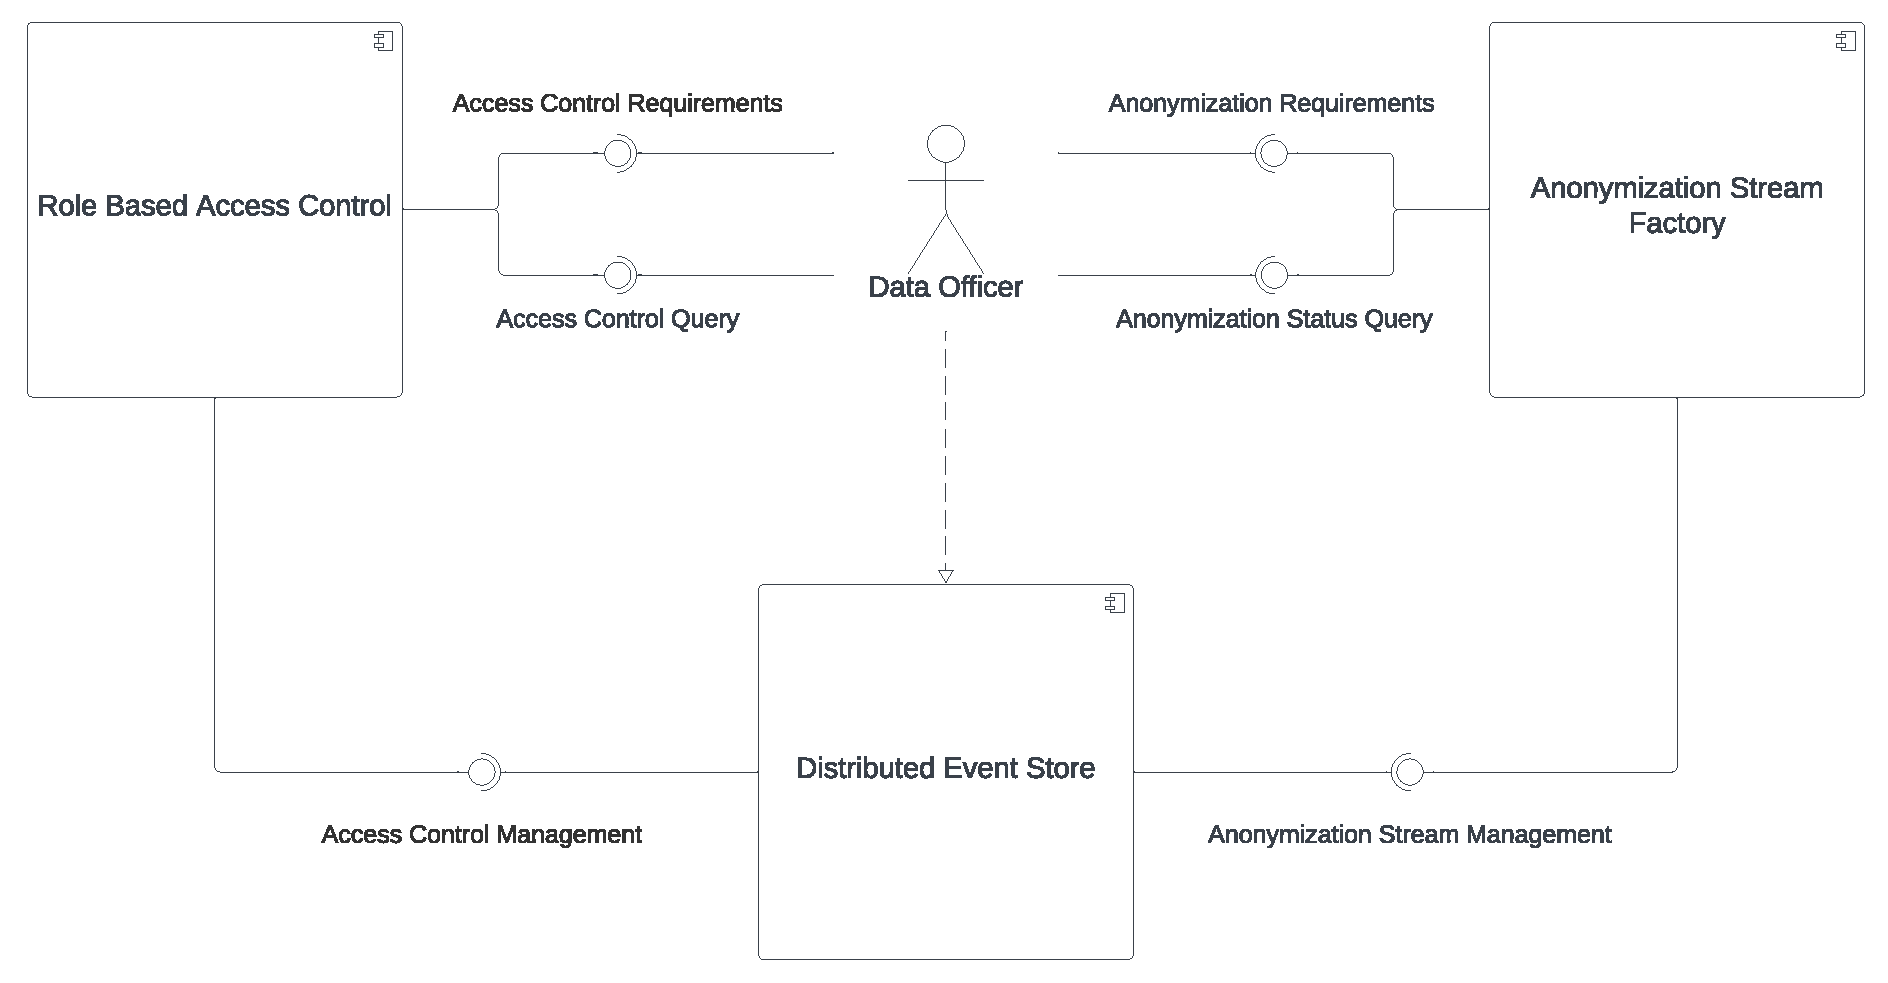
\includegraphics[width=0.8\pdfpagewidth]{img/Component_Diagram.pdf}
    \end{adjustbox}
    \caption{UML Component Diagram of the anonymization system for distributed event stores. \label{fig:componentDiagram}}
\end{figure}

At the center of the architecture, the Data Officer serves as the primary and sole user of the system. The Data Officer interacts with components of the system via interfaces. In the diagram, the interaction points are represented by lines terminating in either circles or semicircles. These symbolize required and provided interfaces respectively. The role of the Data Officer embodies either an individual or a group within an organization responsible for data management. This role, therefore, depends on the \ac{DES} as their primary source of data. The Data Officer is reliant on the proper functionality and accessibility of these stores. This dependency is represented by the dotted arrow in the diagram. The people with the Data Officer role are expected to be technically skilled individuals with extensive knowledge of the data flowing through the \ac{DES}. This is critical as the Data Officer has the authorization to assign and withdraw access control to all consumers and producers of data within the \ac{DES}. Additionally, these people will have to think of and define the levels of anonymization appropriate for their use case, a non-trivial task as we have seen in Section \ref{sec:anon_granularity}. In the context of the anonymization system, however, the Data Officer does not operate directly with the \ac{DES}. Instead, these interactions are abstracted away to two intermediate independent components - one responsible for Role Based Access Control and one we call the Anonymization Stream Factory. They communicate with each other by passing requirements and status updates. These are explicitly two different interactions because of their usage. The requirements are meant to be large one-time occurrences at the setup stage of the operation. They dictate the layout of the initial anonymization structure. During runtime, the Data Officer can monitor the processes through queries. This is the other type of interaction. For the \ac{RBAC}, one can conceptualize the requirements as a collection of individual access control queries. As such the interactions merge on the \ac{RBAC} side of the system. The interactions for the Anonymization Stream Factory paint a similar picture. The two components process these incoming requests. In the case of the requirements, they transform these into a form, which is interpretable by the management component of the \ac{DES}. \par

With a general understanding of the overarching components and interactions, we can look deeper into each component. Figure \ref{fig:component_rbac} provides an in-depth look at the component responsible for enabling \ac{RBAC}. Note that this is not the only possible approach to facilitate role-based access control. 

\begin{figure}[ht]
    \begin{adjustbox}{center}
    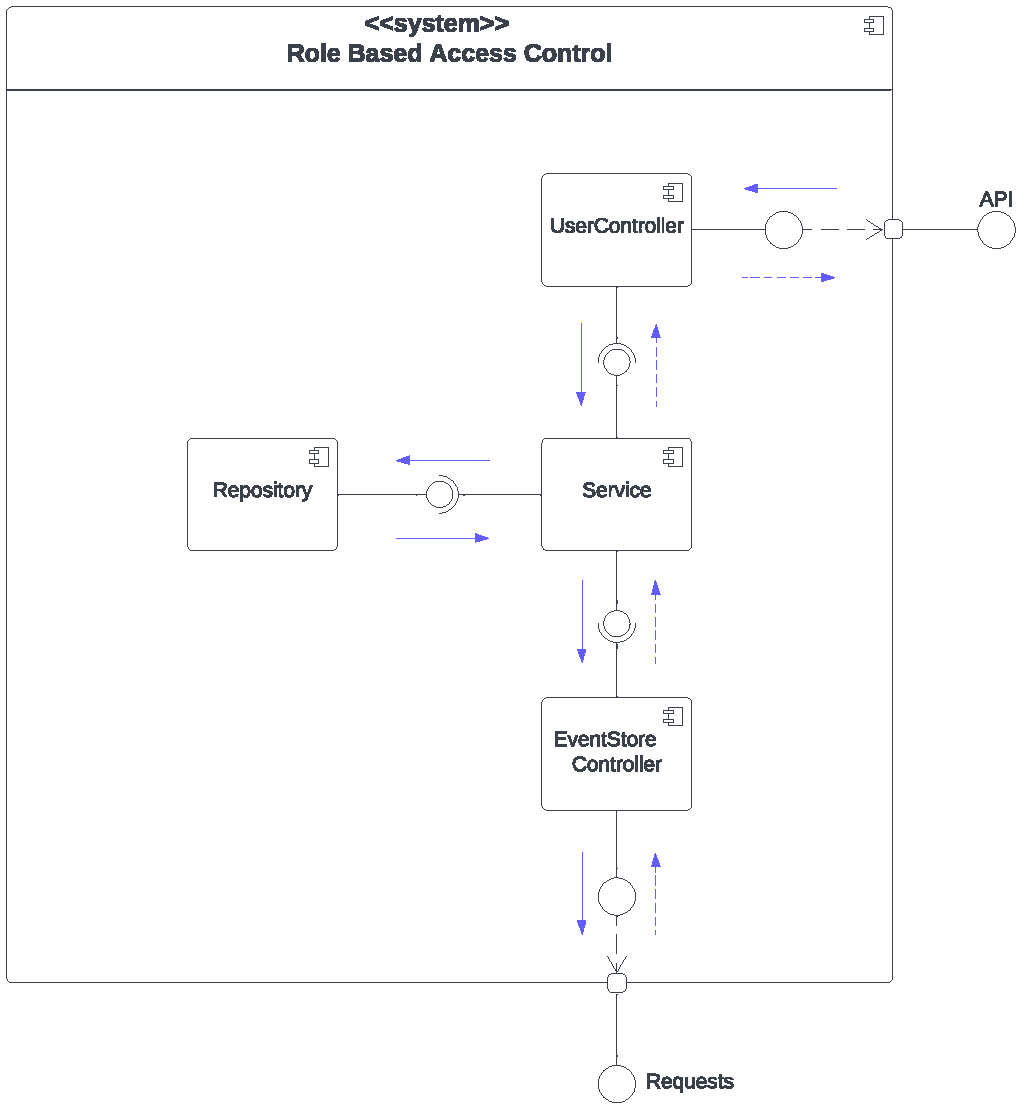
\includegraphics[width=0.7\textwidth]{img/RBAC_Component_Diagram.pdf}
    \end{adjustbox}
    \caption{UML Component Diagram of the component responsible for facilitating Role Based Access Control. Additionally, blue arrows have been added symbolizing data flowing. Dashed lines indicate simple response codes. \label{fig:component_rbac}}
\end{figure}

The Component Diagram shows the system operating with a Controller-Service-Repository setup. The Controller is responsible for interactions with the Client. As there are two Clients, the Data Officer and the Distributed Event Store, two separate controllers distribute the responsibility. Blue arrows in the diagram indicate the data flow. They have been added to the UML diagram to highlight a distinct feature of this system. Data is generally only flowing in one direction. These instructions, provided by the Data Officer, are translated by the RBAC system into requests directed to the \ac{DES}. The only data flowing back are simple responses without payload as illustrated by the dashed arrows. The external interactions are handled by the controllers. These then pass on the data to the service. Here the business logic of the system is executed. Incoming requests are addressed and, either transformed and forwarded to the \ac{DES} or immediately taken care of. Hereby, the repository is utilized. The roles and their access clearance must be saved somewhere. If the \ac{DES} would already have the role and their access clearance, the \ac{RBAC} system would be redundant. As this is not the case the management of roles falls to the responsibility of this component. An API request for the addition of a role would be handled by the \ac{RBAC} component and by this component alone. The modification of a role, however, would need to be forwarded to the \ac{DES} if a user occupies this role. It would convert this role modification into modified Access Control Lists of each user with that role and pass these on. Additions or modifications to users are stored within the component and also forwarded, for analogous reasons. Altogether this leads to an overall better user experience for the Data Officer. They would only have to deal with the abstraction of access control lists in the form of roles, simplifying requests and making them less error-prone in the process. One important additional functionality the \ac{RBAC} component has to offer is the assignment of roles to the consumption of streams. Users will be able to access different versions of the data depending on their role. The access control aspect of this will be managed by this component as well. The functionality of providing differently anonymized versions of data is provided by another component - the Anonymization Stream Factory. \par

The Anonymization Stream Factory is the heart of the system. Its Component Diagram is depicted in Figure \ref{fig:anon_fac_component}. Within this component, the specifications provided by the Data Officer are implemented. After thoroughly analyzing their data needs, a plan detailing the anonymization granularity was formulated and transformed into a comprehensive set of requirements. These requirements are subsequently transmitted to the entry point of the Anonymization Stream Factory. The requirements include all the necessary information of the stream that is supposed to be anonymized. It also includes the wishes for the various levels of anonymization. Together they are sent to the entry point of the anonymization stream factory.\par

\begin{figure}[ht]
    \begin{adjustbox}{center}
    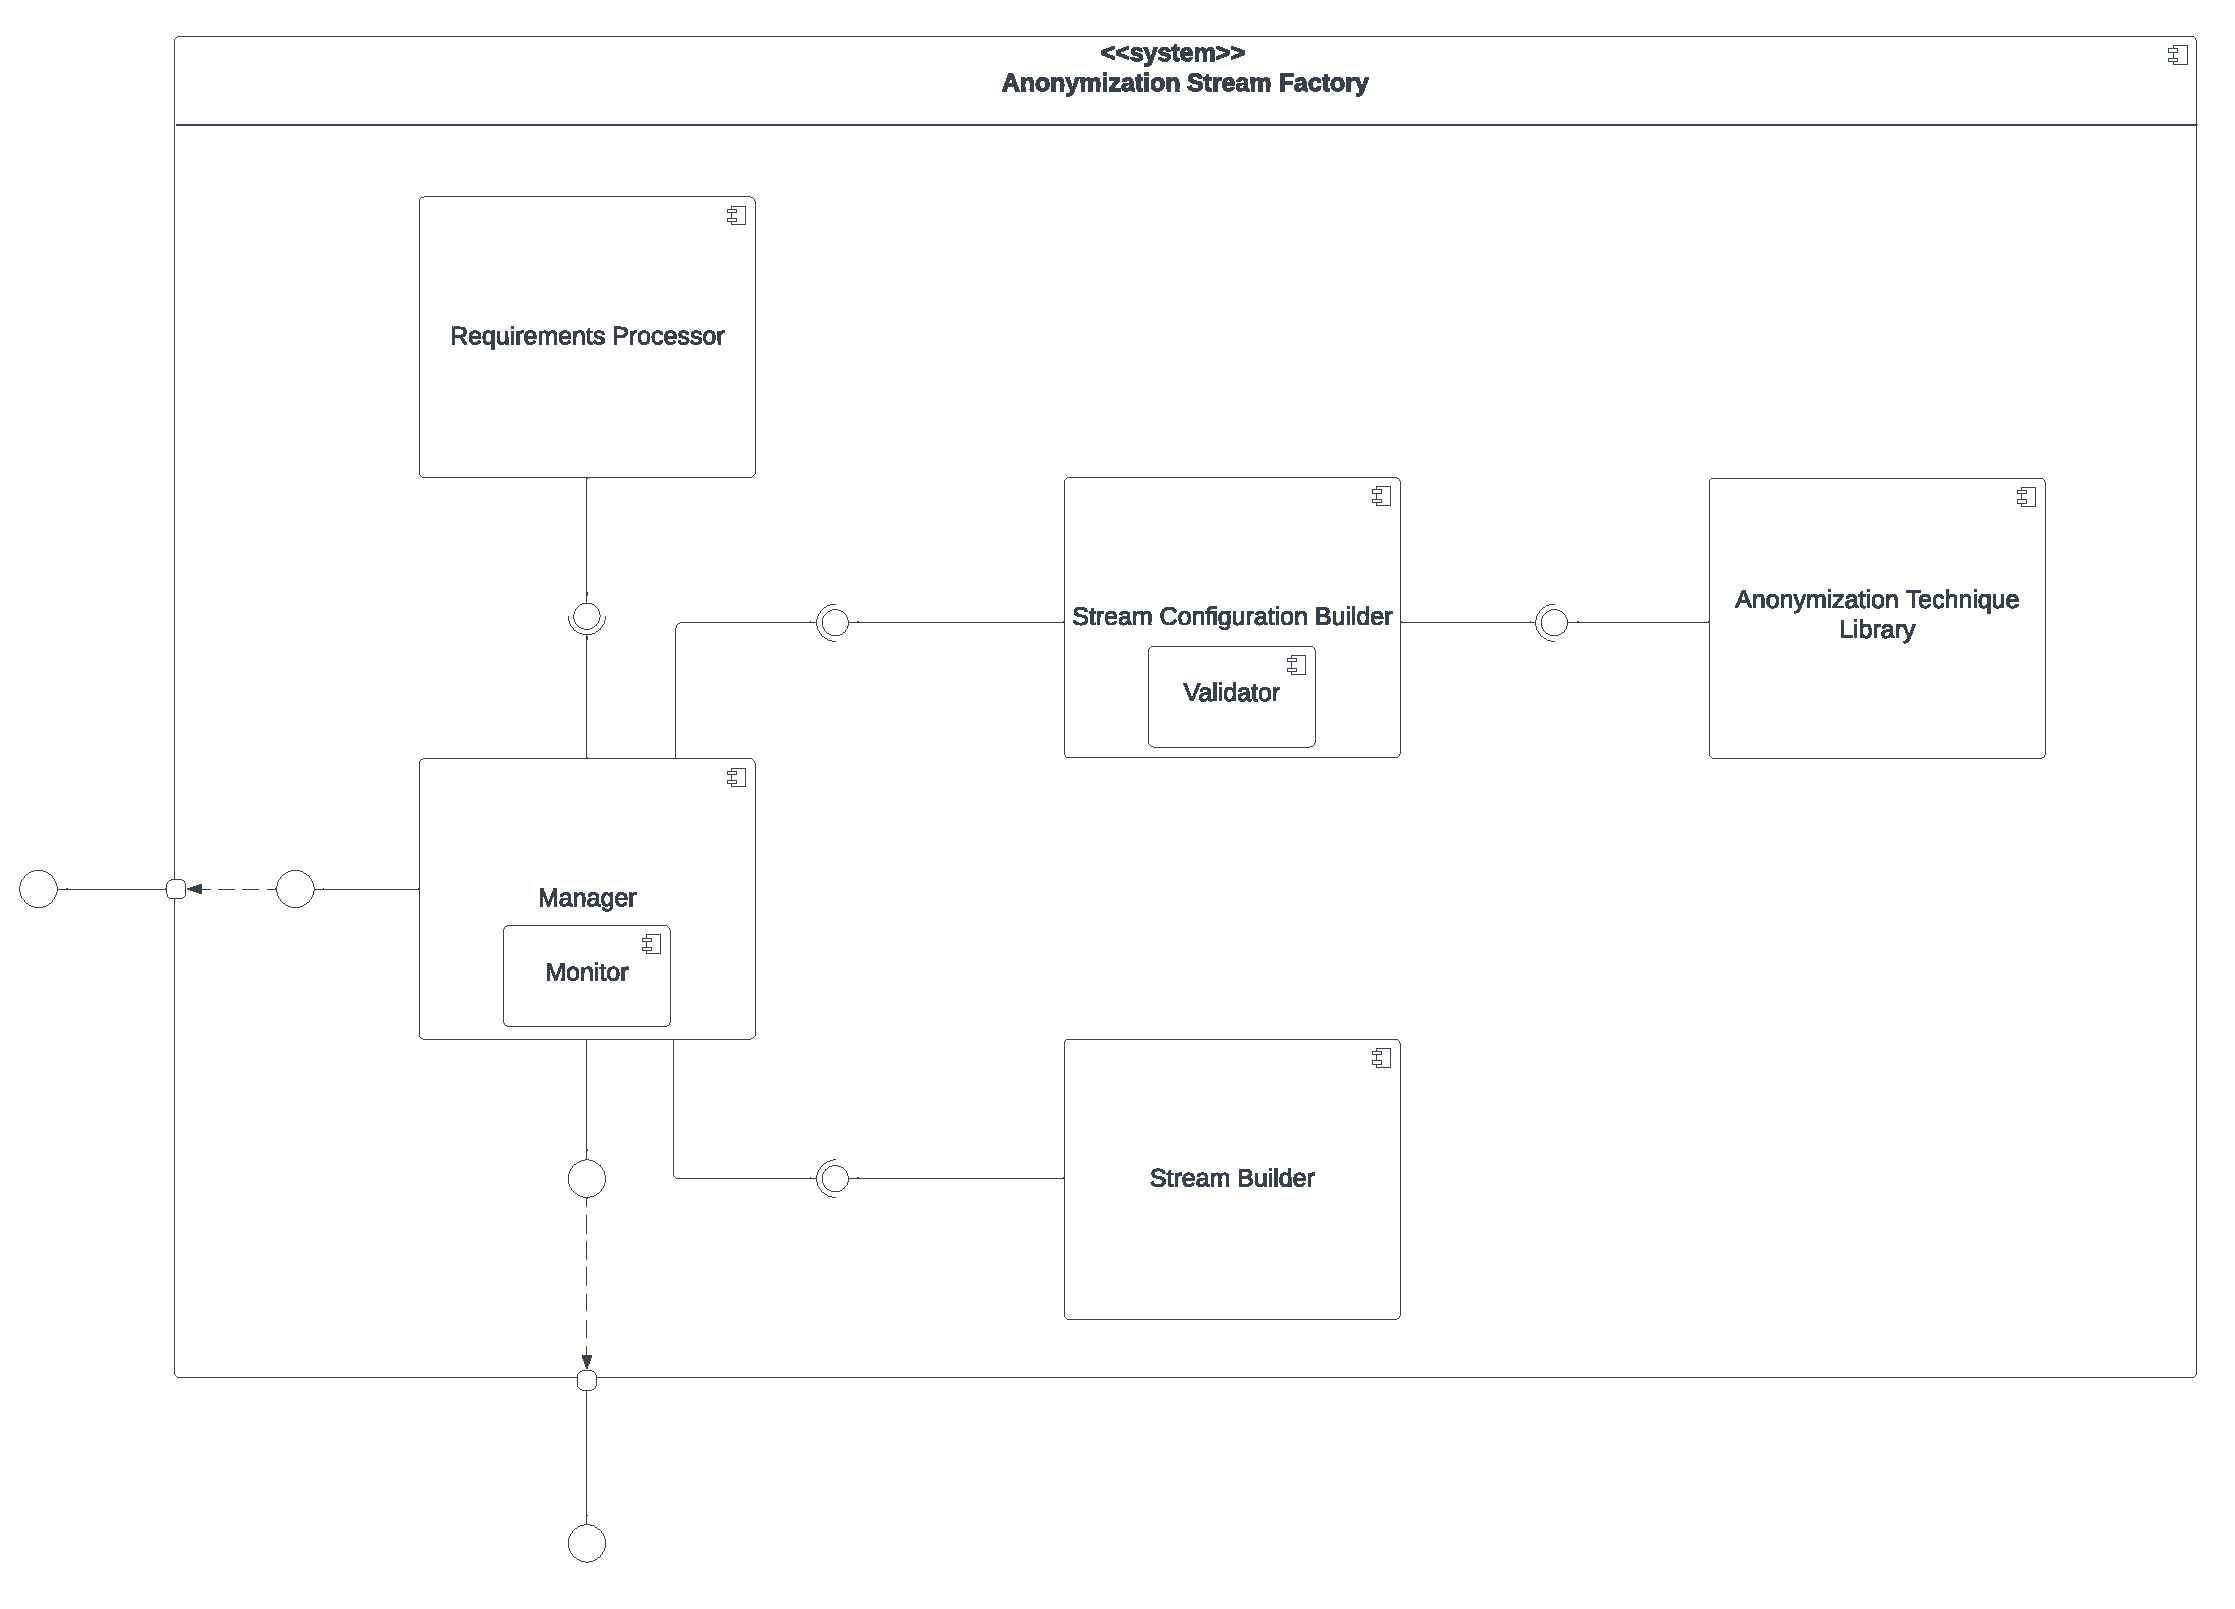
\includegraphics[width=0.8\pdfpagewidth]{img/Anon_Factory_Component_Diagram.pdf}
    \end{adjustbox}
    \caption{UML Component Diagram of the anonymization system for distributed event stores. Additionally, blue arrows have been added symbolizing data flowing. Dashed lines indicate simple response codes. \label{fig:anon_fac_component}}
\end{figure}

Internally, these are received by the system's central component, the Manager. This component is responsible for external communication as well as internal communication. With that, its main task is forwarding data. First, the requirements are passed on to the Requirements Processor. As the requirements are expected to come in one request, These requirements are translated into a format comprehensible to this component and then deconstructed into their parts. Remember, these are the original stream configuration and the various anonymized stream desires. These desires will then be passed individually on to the Stream Configuration Builder. It verifies the availability of the desired anonymization techniques for the stream by interacting with the Anonymization Technique Library. An immutable data component within the system. In Section \ref{sec:anon} we have seen that each anonymization technique can be finetuned through parameters. While these can be syntactically checked with the requirements processor, their semantics need to be validated as well. For this, the configuration builder must include some sort of validation component. The validation must be properly done at this stage as catching these errors should be done before the stream's runtime. They should also be well communicated back to the Data Officer. Regardless of the outcome, the results are relayed back to the Manager. Either with an error message, that is to be forwarded back to the user or with the defined stream configurations. These then can be passed on to the Stream Builder. Here the actual streams are built, they will consume the original data stream and transform it according to the stream configuration, then produce a new anonymized stream. This ready-to-go stream will be passed back again to the Manager. Subsequently, the Manager forwards the processed stream to the \ac{DES}. It should either be able to monitor the status of the streams by itself or answer the status queries by the data officer with forwarded messages from the \ac{DES}. \par

Finally, let us take a look at the internal architecture of the Distributed Event Store. Figure \ref{fig:des_component} shows its Component Diagram. At the core are the individual Event Stores. Each is responsible for storing and managing data (in this context also often to referred as "Events"). They are distributed, forming a loose cluster of individually not connected stores. They can be spread across multiple physical machines and even different geographical locations. The Event Stores are controlled by the administration component of the system. It monitors and logs the stores as well as gives commands like adding or removing individual event stores. The administration also decides on the partitioning and aggregation logic. The main benefits of a distributed system are scalability and reliability. It accomplishes horizontal scalability with ease through the extension of additional event stores. The workload is then balanced across these stores to mitigate bottlenecks. Reliability is facilitated through replicability. If any one event store fails, there is another with replicated data, which can take its place until the original event store is back online. This leads to increased fault tolerance, data durability, and higher availability. All this relies on the proper replication and distribution logic. The strategy is chosen by the Administration and forwarded to the Partitioner component to put into effect. It takes the data collected by the producers and shards it e.g. splits it into multiple pieces. Shards are replicated and sent to other destinations. The Aggregator does the composite process. From the Administration, it is familiar with the distribution logic and can piece together the data from multiple sources into one output. This output is relayed to the consumers of the data.



\begin{figure}[ht]
    \begin{adjustbox}{center}
    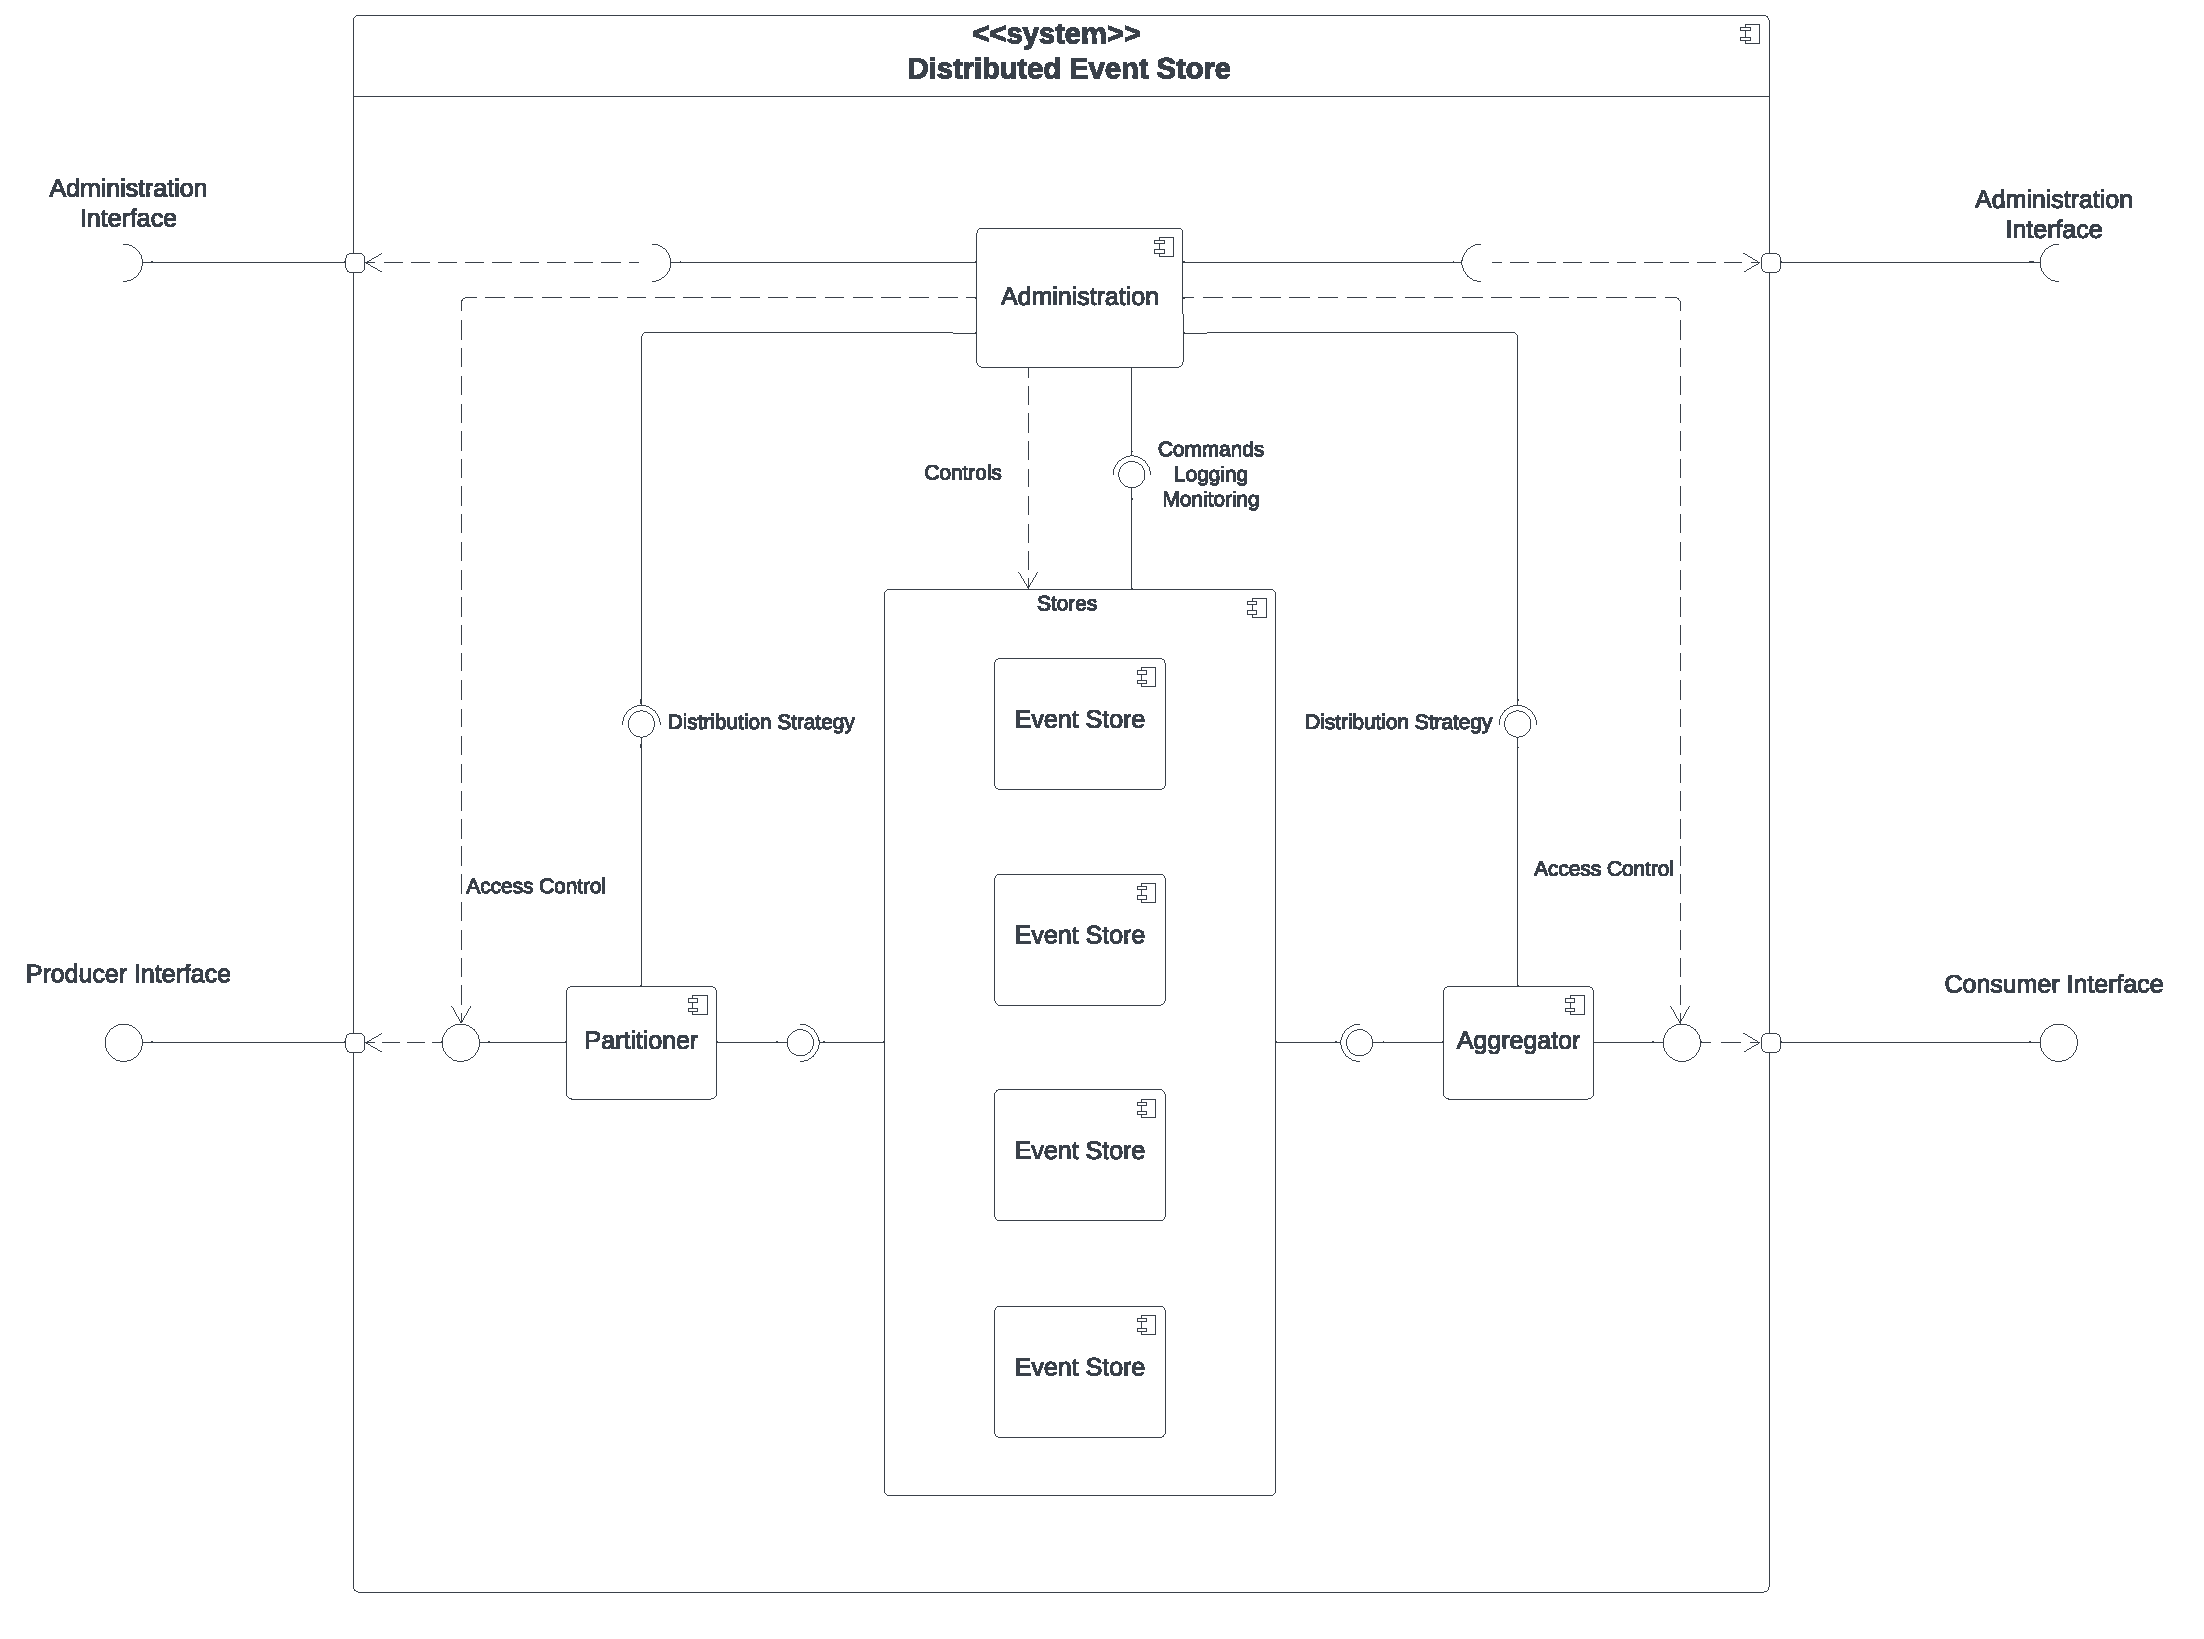
\includegraphics[width=0.8\pdfpagewidth]{img/DES_Component_Diagram.pdf}
    \end{adjustbox}
    \caption{Architecture of a Distributed Event Store illustrated with a UML Component Diagram. \label{fig:des_component}}
\end{figure}

The Administration component is configurable from the outside through an interface. Normally, there is only one expected interface. The reason for the two interfaces shown in the diagram is simply due to it being a part of a bigger Component Diagram shown in Figure \ref{fig:componentDiagram}. It is administrated from two other components, the \ac{RBAC} system and the Anonymization Stream Factory, both dictated by the Data Officer. The full Component Diagram spans multiple pages and can be found in Appendix \ref{app:component_diagram}. In reality, it would be safe to assume that the other components interact with the Distributed Event Store through one administration interface. Through this interface, for example, access control can be assigned or data streams added. The access control would then be enforced at the system's data ports. 

\subsection{Functional Requirements}

The architectural layout presented until this point describes the system as a whole, its components, and their interactions, thereby serving as a blueprint for the envisioned infrastructure. Let us translate this vision into actionable and measurable goals: \par

\begin{enumerate}
    \item \textbf{Data Stream Integration}\\ Distributed Event Stores are specialized towards operating on streaming data; appropriate integration is essential to the success of the system. The system is anticipated to receive streaming data as the input that requires anonymization. Consequently, the anonymized output data must likewise be in a streaming format. The system must facilitate the ingestion, processing, and management of data streams in real-time, ensuring both the efficiency and reliability of data handling. 
    \item \textbf{Administrative Control}\\ The goal of the system is to provide granular anonymization to its user, the Data Officer. Here, the system must provide tools for the Data Officer to govern the system's operation. This specifically includes access control management and oversight of the data processing pipeline. The system must incorporate robust monitoring tools and provide interfaces for the user.
    \item \textbf{Adaptability}\\ With any large software endeavor comes changes in requirements over time. The system must be adaptable to that change. New anonymization techniques must be addable to the system. Existing ones must be customizable. It must be possible to modify the system ports to enable connections to different distributed event stores. The system's architecture must be designed with flexibility at its core, accommodating changes in requirements and technological advancements with minimal disruption.
\end{enumerate}


\subsection{Non-functional Requirements}
Finally, let us address the non-functional requirements. Although non-functional requirements do not dictate system functionality, they are imperative for the operational integrity of the system. Reiterating that the strengths of Distributed Event Stores lie in their ability to efficiently handle large amounts of data in real-time, the addition of the proposed system mustn't diminish these. Therefore, the three main non-functional requirements of the system are essential to maintain the strengths of the underlying distributed event stores: 

\begin{enumerate}
    \item \textbf{Performance}\\ The system should minimize performance overhead. This can be evaluating the latency and throughput with and without the anonymization system in place. Additionally, storage is always a concern. However, given the fact that the system's central idea is duplicating the data and providing different anonymized versions through different streams, much more storage capacity can be expected. 
    \item \textbf{Reliability}\\ The system must ensure the availability of anonymized data counterparts concurrently with non-anonymized data. System failure carries significant risks. Furthermore, it must be guaranteed that non-anonymized data is under the strict proposed access control rules. The plain text data being available to unauthorized persons would jeopardize the entire system. 
    \item \textbf{Scalability}\\ It should be possible to easily scale the system horizontally, mirroring the core attributes of distributed systems. Accommodating increasing data loads and parallel processing demands without compromising the efficiency of the anonymization process, is what the system should strive to do.
\end{enumerate}

